\documentclass[preprint, 3p,
authoryear]{elsarticle} %review=doublespace preprint=single 5p=2 column
%%% Begin My package additions %%%%%%%%%%%%%%%%%%%

\usepackage[hyphens]{url}

  \journal{An awesome journal} % Sets Journal name

\usepackage{lineno} % add

\usepackage{graphicx}
%%%%%%%%%%%%%%%% end my additions to header

\usepackage[T1]{fontenc}
\usepackage{lmodern}
\usepackage{amssymb,amsmath}
\usepackage{ifxetex,ifluatex}
\usepackage{fixltx2e} % provides \textsubscript
% use upquote if available, for straight quotes in verbatim environments
\IfFileExists{upquote.sty}{\usepackage{upquote}}{}
\ifnum 0\ifxetex 1\fi\ifluatex 1\fi=0 % if pdftex
  \usepackage[utf8]{inputenc}
\else % if luatex or xelatex
  \usepackage{fontspec}
  \ifxetex
    \usepackage{xltxtra,xunicode}
  \fi
  \defaultfontfeatures{Mapping=tex-text,Scale=MatchLowercase}
  \newcommand{\euro}{€}
\fi
% use microtype if available
\IfFileExists{microtype.sty}{\usepackage{microtype}}{}
\usepackage[]{natbib}
\bibliographystyle{plainnat}

\ifxetex
  \usepackage[setpagesize=false, % page size defined by xetex
              unicode=false, % unicode breaks when used with xetex
              xetex]{hyperref}
\else
  \usepackage[unicode=true]{hyperref}
\fi
\hypersetup{breaklinks=true,
            bookmarks=true,
            pdfauthor={},
            pdftitle={Short Paper},
            colorlinks=false,
            urlcolor=blue,
            linkcolor=magenta,
            pdfborder={0 0 0}}

\setcounter{secnumdepth}{5}
% Pandoc toggle for numbering sections (defaults to be off)

% Pandoc syntax highlighting
\usepackage{color}
\usepackage{fancyvrb}
\newcommand{\VerbBar}{|}
\newcommand{\VERB}{\Verb[commandchars=\\\{\}]}
\DefineVerbatimEnvironment{Highlighting}{Verbatim}{commandchars=\\\{\}}
% Add ',fontsize=\small' for more characters per line
\usepackage{framed}
\definecolor{shadecolor}{RGB}{248,248,248}
\newenvironment{Shaded}{\begin{snugshade}}{\end{snugshade}}
\newcommand{\AlertTok}[1]{\textcolor[rgb]{0.94,0.16,0.16}{#1}}
\newcommand{\AnnotationTok}[1]{\textcolor[rgb]{0.56,0.35,0.01}{\textbf{\textit{#1}}}}
\newcommand{\AttributeTok}[1]{\textcolor[rgb]{0.77,0.63,0.00}{#1}}
\newcommand{\BaseNTok}[1]{\textcolor[rgb]{0.00,0.00,0.81}{#1}}
\newcommand{\BuiltInTok}[1]{#1}
\newcommand{\CharTok}[1]{\textcolor[rgb]{0.31,0.60,0.02}{#1}}
\newcommand{\CommentTok}[1]{\textcolor[rgb]{0.56,0.35,0.01}{\textit{#1}}}
\newcommand{\CommentVarTok}[1]{\textcolor[rgb]{0.56,0.35,0.01}{\textbf{\textit{#1}}}}
\newcommand{\ConstantTok}[1]{\textcolor[rgb]{0.00,0.00,0.00}{#1}}
\newcommand{\ControlFlowTok}[1]{\textcolor[rgb]{0.13,0.29,0.53}{\textbf{#1}}}
\newcommand{\DataTypeTok}[1]{\textcolor[rgb]{0.13,0.29,0.53}{#1}}
\newcommand{\DecValTok}[1]{\textcolor[rgb]{0.00,0.00,0.81}{#1}}
\newcommand{\DocumentationTok}[1]{\textcolor[rgb]{0.56,0.35,0.01}{\textbf{\textit{#1}}}}
\newcommand{\ErrorTok}[1]{\textcolor[rgb]{0.64,0.00,0.00}{\textbf{#1}}}
\newcommand{\ExtensionTok}[1]{#1}
\newcommand{\FloatTok}[1]{\textcolor[rgb]{0.00,0.00,0.81}{#1}}
\newcommand{\FunctionTok}[1]{\textcolor[rgb]{0.00,0.00,0.00}{#1}}
\newcommand{\ImportTok}[1]{#1}
\newcommand{\InformationTok}[1]{\textcolor[rgb]{0.56,0.35,0.01}{\textbf{\textit{#1}}}}
\newcommand{\KeywordTok}[1]{\textcolor[rgb]{0.13,0.29,0.53}{\textbf{#1}}}
\newcommand{\NormalTok}[1]{#1}
\newcommand{\OperatorTok}[1]{\textcolor[rgb]{0.81,0.36,0.00}{\textbf{#1}}}
\newcommand{\OtherTok}[1]{\textcolor[rgb]{0.56,0.35,0.01}{#1}}
\newcommand{\PreprocessorTok}[1]{\textcolor[rgb]{0.56,0.35,0.01}{\textit{#1}}}
\newcommand{\RegionMarkerTok}[1]{#1}
\newcommand{\SpecialCharTok}[1]{\textcolor[rgb]{0.00,0.00,0.00}{#1}}
\newcommand{\SpecialStringTok}[1]{\textcolor[rgb]{0.31,0.60,0.02}{#1}}
\newcommand{\StringTok}[1]{\textcolor[rgb]{0.31,0.60,0.02}{#1}}
\newcommand{\VariableTok}[1]{\textcolor[rgb]{0.00,0.00,0.00}{#1}}
\newcommand{\VerbatimStringTok}[1]{\textcolor[rgb]{0.31,0.60,0.02}{#1}}
\newcommand{\WarningTok}[1]{\textcolor[rgb]{0.56,0.35,0.01}{\textbf{\textit{#1}}}}

% tightlist command for lists without linebreak
\providecommand{\tightlist}{%
  \setlength{\itemsep}{0pt}\setlength{\parskip}{0pt}}

% From pandoc table feature
\usepackage{longtable,booktabs,array}
\usepackage{calc} % for calculating minipage widths
% Correct order of tables after \paragraph or \subparagraph
\usepackage{etoolbox}
\makeatletter
\patchcmd\longtable{\par}{\if@noskipsec\mbox{}\fi\par}{}{}
\makeatother
% Allow footnotes in longtable head/foot
\IfFileExists{footnotehyper.sty}{\usepackage{footnotehyper}}{\usepackage{footnote}}
\makesavenoteenv{longtable}





\begin{document}


\begin{frontmatter}

  \title{Short Paper}
    \author[Some Institute of Technology]{Alice Anonymous%
  \corref{cor1}%
  \fnref{1}}
   \ead{alice@example.com} 
    \author[Another University]{Bob Security%
  %
  }
   \ead{bob@example.com} 
    \author[Another University]{Cat Memes%
  %
  \fnref{2}}
   \ead{cat@example.com} 
    \author[Some Institute of Technology]{Derek Zoolander%
  %
  \fnref{2}}
   \ead{derek@example.com} 
      \affiliation[Some Institute of Technology]{Department, Street,
City, State, Zip}
    \affiliation[Another University]{Department, Street, City, State,
Zip}
    \cortext[cor1]{Corresponding author}
    \fntext[1]{This is the first author footnote.}
    \fntext[2]{Another author footnote.}
  
  \begin{abstract}
  This is the abstract. It consists of two paragraphs.
  \end{abstract}
    \begin{keyword}
    keyword1 \sep 
    keyword2
  \end{keyword}
  
 \end{frontmatter}

Please make sure that your manuscript follows the guidelines in the
Guide for Authors of the relevant journal. It is not necessary to
typeset your manuscript in exactly the same way as an article, unless
you are submitting to a camera-ready copy (CRC) journal.

For detailed instructions regarding the elsevier article class, see
\url{https://www.elsevier.com/authors/policies-and-guidelines/latex-instructions}

\hypertarget{bibliography-styles}{%
\section{Bibliography styles}\label{bibliography-styles}}

Here are two sample references: \citep{Feynman1963118, Dirac1953888}
\citet{vandijk2006}.

By default, natbib will be used with the \texttt{authoryear} style, set
in \texttt{classoption} variable in YAML. You can sets extra options
with \texttt{natbiboptions} variable in YAML header. Example

\begin{Shaded}
\begin{Highlighting}[]
\FunctionTok{natbiboptions}\KeywordTok{:}\AttributeTok{ longnamesfirst,angle,semicolon}
\end{Highlighting}
\end{Shaded}

There are various more specific bibliography styles available at
\url{https://support.stmdocs.in/wiki/index.php?title=Model-wise_bibliographic_style_files}.
To use one of these, add it in the header using, for example,
\texttt{biblio-style:\ model1-num-names}.

\hypertarget{using-csl}{%
\subsection{Using CSL}\label{using-csl}}

If \texttt{citation\_package} is set to \texttt{default} in
\texttt{elsevier\_article()}, then pandoc is used for citations instead
of \texttt{natbib}. In this case, the \texttt{csl} option is used to
format the references. Alternative \texttt{csl} files are available from
\url{https://www.zotero.org/styles?q=elsevier}. These can be downloaded
and stored locally, or the url can be used as in the example header.

\hypertarget{equations}{%
\section{Equations}\label{equations}}

Here is an equation: \[ 
  f_{X}(x) = \left(\frac{\alpha}{\beta}\right)
  \left(\frac{x}{\beta}\right)^{\alpha-1}
  e^{-\left(\frac{x}{\beta}\right)^{\alpha}}; 
  \alpha,\beta,x > 0 .
\]

Here is another: \begin{align}
  a^2+b^2=c^2.
\end{align}

Inline equations: \(\sum_{i = 2}^\infty\{\alpha_i^\beta\}\)

\hypertarget{figures-and-tables}{%
\section{Figures and tables}\label{figures-and-tables}}

Figure \ref{fig2} is generated using an R chunk.

\begin{figure}

{\centering 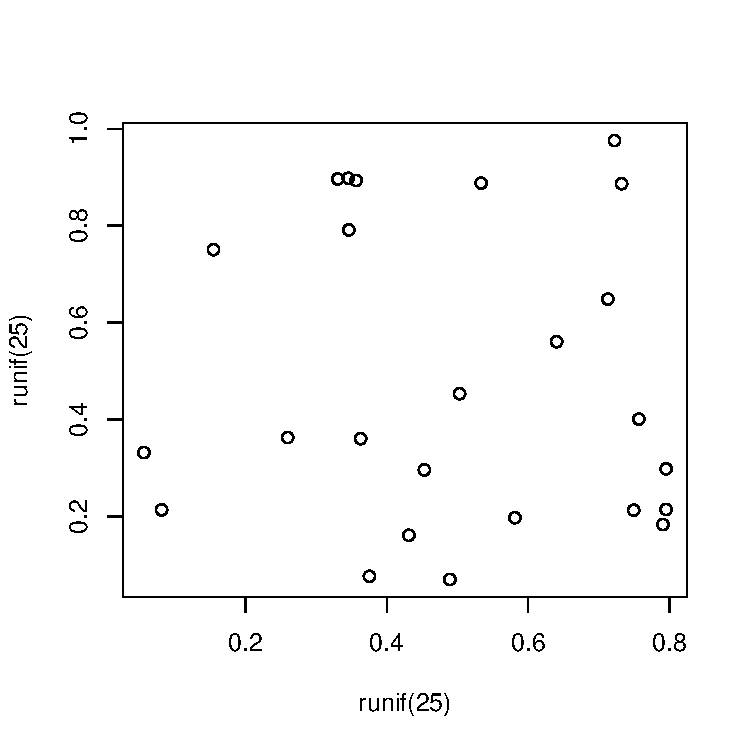
\includegraphics[width=0.5\linewidth]{APA-test_files/figure-latex/fig2-1} 

}

\caption{\label{fig2}A meaningless scatterplot.}\label{fig:fig2}
\end{figure}

\hypertarget{tables-coming-from-r}{%
\section{Tables coming from R}\label{tables-coming-from-r}}

Tables can also be generated using R chunks, as shown in Table
\ref{tab1} for example.

\begin{Shaded}
\begin{Highlighting}[]
\NormalTok{knitr}\SpecialCharTok{::}\FunctionTok{kable}\NormalTok{(}\FunctionTok{head}\NormalTok{(mtcars)[,}\DecValTok{1}\SpecialCharTok{:}\DecValTok{4}\NormalTok{], }
    \AttributeTok{caption =} \StringTok{"}\SpecialCharTok{\textbackslash{}\textbackslash{}}\StringTok{label\{tab1\}Caption centered above table"}
\NormalTok{)}
\end{Highlighting}
\end{Shaded}

\begin{longtable}[]{@{}lrrrr@{}}
\caption{\label{tab1}Caption centered above table}\tabularnewline
\toprule()
& mpg & cyl & disp & hp \\
\midrule()
\endfirsthead
\toprule()
& mpg & cyl & disp & hp \\
\midrule()
\endhead
Mazda RX4 & 21.0 & 6 & 160 & 110 \\
Mazda RX4 Wag & 21.0 & 6 & 160 & 110 \\
Datsun 710 & 22.8 & 4 & 108 & 93 \\
Hornet 4 Drive & 21.4 & 6 & 258 & 110 \\
Hornet Sportabout & 18.7 & 8 & 360 & 175 \\
Valiant & 18.1 & 6 & 225 & 105 \\
\bottomrule()
\end{longtable}

\renewcommand\refname{References}
\bibliography{mybibfile.bib}


\end{document}
